\section{Final Velocity Model}
\eqref{eq:Totaltorquewithcurrentexpression} along with the transfer function for the mechanical part, \eqref{eq:mechanicalTransFerfunction}, delivers the information needed to make a visual representation of the velocity model. The input is the supply voltage, \si{U_a(s)} delivered to the motor and the output is the vehicles velocity, \si{V(s)}, see \figref{fig:BlockDiagramDrivetrainComplicated}. 
%
\begin{figure}[H]
	\centering
	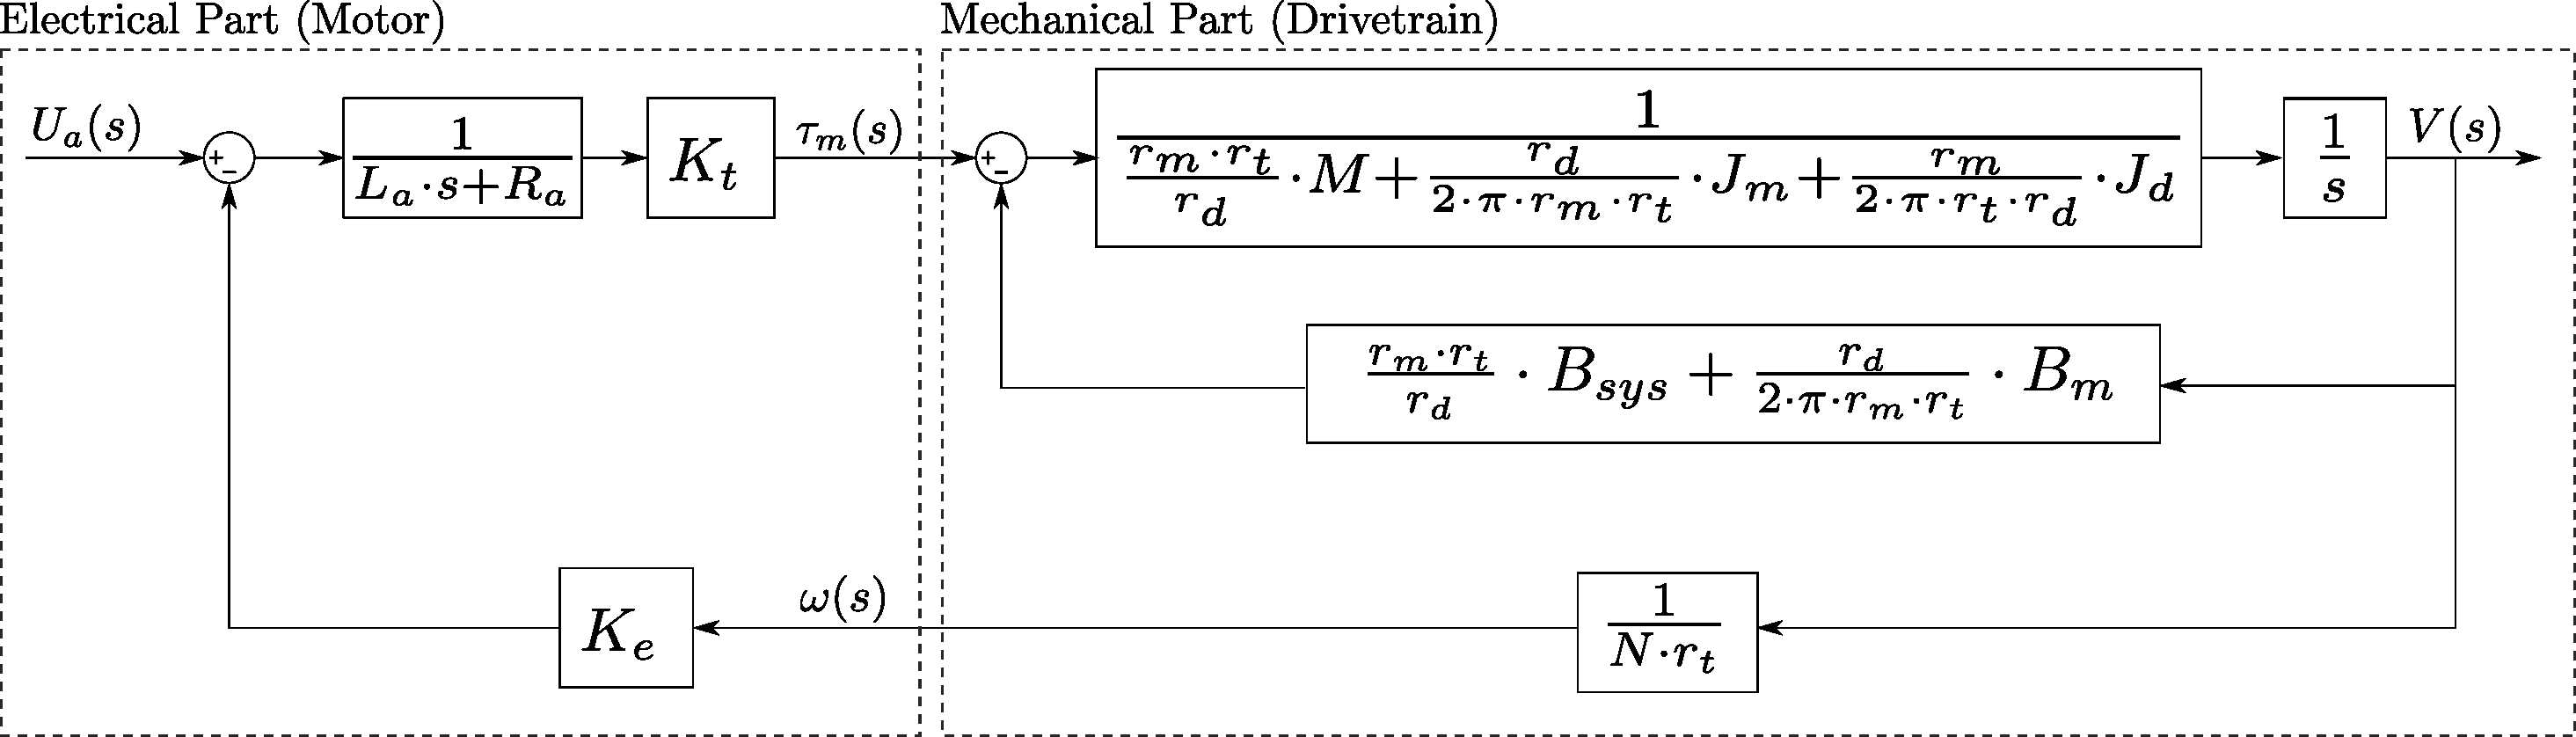
\includegraphics[width=\textwidth]{figures/totalVelocityModelDiagramComplicated.pdf}
	\caption{A block diagram of the combined drivetrain}
	\label{fig:BlockDiagramDrivetrainComplicated}
\end{figure}
%
Less complicated model:

\begin{figure}[H]
	\centering
	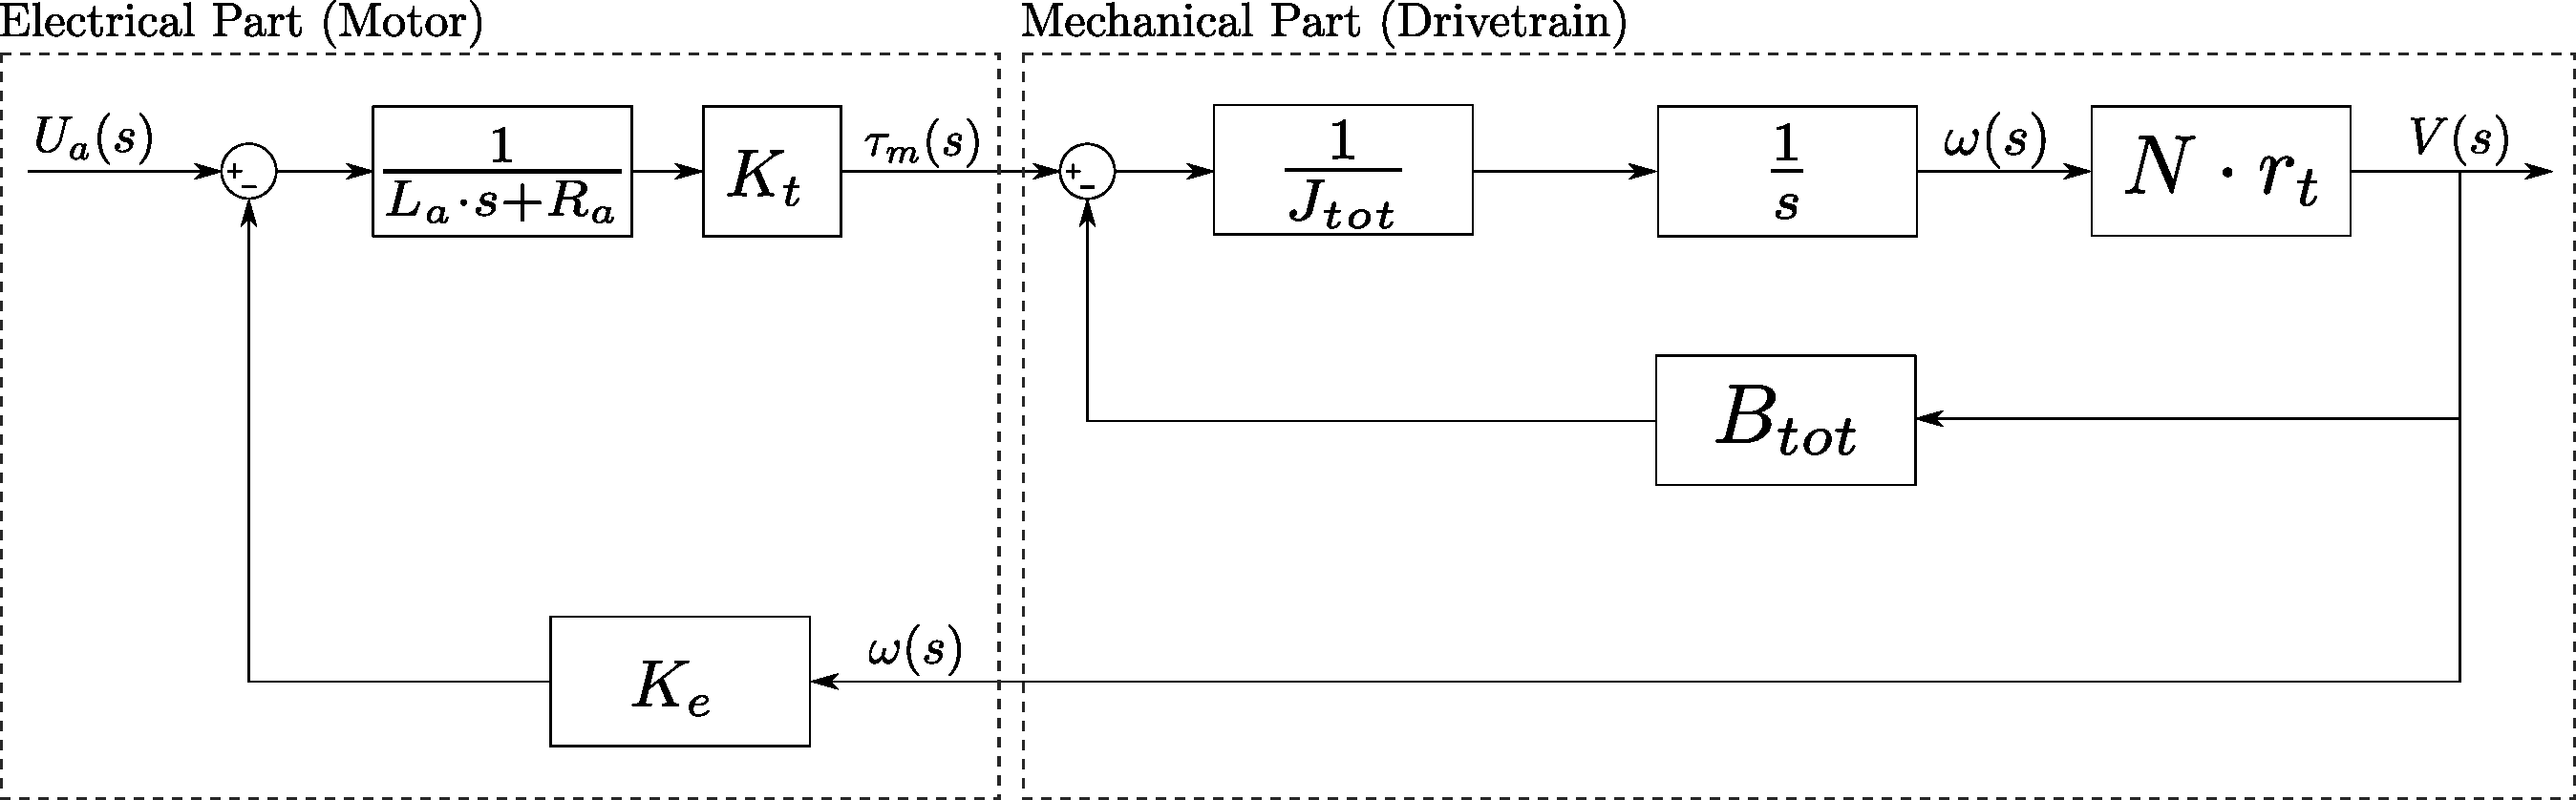
\includegraphics[width=\textwidth]{figures/totalVelocityModelDiagramNotComplicated.pdf}
	\caption{A block diagram of the combined drivetrain}
	\label{fig:BlockDiagramDrivetrainNotComplicated}
\end{figure}